\documentclass[10pt,a4paper]{article}
\usepackage[margin=18mm]{geometry}
\usepackage[T1]{fontenc}
\usepackage{lmodern,graphicx,booktabs,amsmath,xcolor}
\usepackage[hidelinks]{hyperref}
\setlength{\parindent}{0pt}
\setlength{\parskip}{6pt}
\pagestyle{plain}
\begin{document}
{\Large\bfseries A genuine CM19 genus-three source over F7}\par
23 November 2026 \quad Native correctness result; unsigned [pcc:unverified]

\textbf{Outcome.} The separately fixed primary-derived plane quartic is
smooth and has Weil polynomial $(T^2+3T+7)^3$. Its rational Jacobian has
order $11^3=1331$. This supplies an actual curve in the desired unpolarized
isogeny class; explicit polarized-model and nontrivial-kernel maps remain open.
The completed fixed250 F5 negative stays unchanged.

\[
 C_7:(Z^2+6X^2+3XY+Y^2)^2=Y(X^3+2XY^2+6Y^3).
\]
The elliptic quotient is $E_7:v^2=x^3+2x+6$, with
$v=z^2+6x^2+3x+1$. Its trace is $-3$ and rational order 11.

\begin{center}
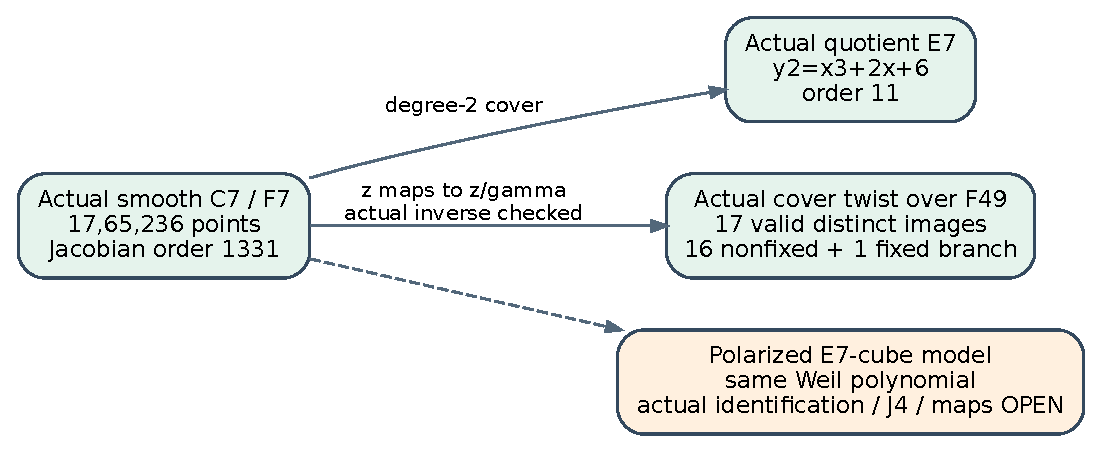
\includegraphics[width=\linewidth,height=61mm,keepaspectratio]{source.pdf}
\end{center}

\begin{center}
\begin{tabular}{@{}lrrrr@{}}
\toprule
Model & $N_1$ & $N_2$ & $N_3$ & Rational group order\\
\midrule
$C_7$, $\kappa=1$ & 17 & 65 & 236 & $1331$ (Jacobian)\\
Cover twist, $\kappa=3$ & 5 & 65 & 380 & $275$ (Jacobian)\\
$E_7$ & 11 & 55 & 308 & $11$ (elliptic)\\
\bottomrule
\end{tabular}
\end{center}

Native integer Newton identities give the full degree-six polynomials
\[
\begin{aligned}
 P_{C_7}&:\ [343,441,336,153,48,9,1],\\
 P_{\rm twist}&:\ [343,-147,84,-15,12,-3,1],
\end{aligned}
\]
in ascending coefficient order. Both contain $P_E=T^2+3T+7$;
$P_{C_7}=P_E^3$ has mod-2 polynomial $\Phi_3^3$.

\textbf{A working descent control.}
In $\mathbf F_{49}=\mathbf F_7[b]/(b^2-3)$, $\gamma=b$ has
$\gamma^7=-\gamma$. The actual map $z'=z/\gamma$ gives 17 distinct
valid images on the cover twist and has an actual inverse. Frobenius equals
the deck involution. Exactly 16 images fail F7 descent; the branch point
$[1:1:0]$ remains fixed. All source/image/Frobenius points are printed.
This curve-map control does not implement Jacobian four-torsion arithmetic.

\textbf{Evidence.} Source \texttt{0b9b506b}; full result \texttt{89d7b471};
unsigned claim \texttt{PCC-20261123-180c4c}. [pcc:unverified]
\newpage
{\Large\bfseries Primary identity, exact controls and research boundary}\par

\textbf{A genuine smooth source.}
Ritzenthaler's 2010 Example 1 gives the rational CM19 quartic. Native
multivariate arithmetic checks every one of the 15 homogeneous degree-four
coefficients after $X=V+3W$, $Y=W$, $Z=2U$, with scale 2. An actual
primary $W^4$ coefficient mutation fails, and pristine restoration passes.
The branch polynomial $h=x^4+4x+2$ has exact gcd$(h,h')=1$ and independent
Sylvester nullity zero. The singular $x^2$ control fails both tests.
The written geometric smoothness criterion therefore gives a smooth plane
quartic, hence a genuine nonhyperelliptic genus-three curve.

\textbf{Independent counts and field controls.}
Every projective point is counted by an expanded direct evaluator and by
independent elliptic-fibre square-root histograms, including infinity.
Both routes agree for both $\kappa$ values over F7, F49 and F343. Paired
odd-degree counts sum to 22 and 616; degree-two counts agree. Altering
$N_3$ by $+3$ rejects the elliptic factor in each row, and restoration passes.
All three native fields pass complete pair/triple, inverse and Frobenius
controls. F49 uses $b^2=3$; F343 uses $t^3+2t+1=0$. The original F5
population was not replayed.

\textbf{Implementation and custody.}
All seven strict B phases exit zero, with unchanged source/tool/runtime and
qualifier guards. Rust 1.99.1, edition 2021, warnings denied, overflow/debug
assertions, one worker, 2 GiB and 120 seconds per phase. All 18 complete
locked inputs were read back before the call. The first strict format
negative has its complete 5977-byte diagnostic and original metadata;
neither compiler nor native source qualification ran before its B repair.

All 38 small B records are public, and all 43 result-commit files were
fully read back. Whole native stdout is 3373 bytes, SHA256
\texttt{6bcb4141\ldots c0b9db08}. The original 4656584-byte ELF remains in
temporary custody pending approved-store or CI retention. This is a local
development correctness qualification, with no timing or DLP claim.

\textbf{What still needs construction.}
The point counts establish an unpolarized isogeny class. They do not
identify the actual principal polarization with a chosen CM19 Hermitian
lattice. That primary-source/base-field bridge must be independently
validated before transporting an abstract mixed kernel. Actual $J[4]$,
the nontrivial quotient map and target Jacobian/Serre descent, original
elliptic subgroup preservation and complete strongest-reference cold costs
remain open. No cryptographic-size solve, independent replay or generic
Mathlib theorem is established here.

\textbf{Sources and standing.}
\href{https://github.com/isogeny-labs/crypto/tree/0b9b506bc035d8ada6a111702b2ae3145e65deb6/research/chained_genus3_quartic_20261123/cm19_f7}{Complete frozen source/protocol}
and
\href{https://github.com/isogeny-labs/crypto/tree/89d7b471a53c564f9e0368a83315d5acbdd23218/research/chained_genus3_quartic_20261123/cm19_f7}{full result/raw records}.
Primary: Ritzenthaler, DOI 10.1112/S1461157009000576, Example 1,
Table 2 and Section 4.4. KB/Conductor unavailable; no novelty clearance.
Existing paid STOP, vault, owners, experiment, formal, CI and merge gates
remain binding. All scientific findings are unsigned. [pcc:unverified]
\end{document}
